% -*- coding: utf-8; -*-
\chapter{Objetivos}
\label{cha:Objetivos}

Como dito no capítulo anterior, o ramo de imagens médicas é extramente importante para a medicina e aplicar técnicas de inteligência artificial para automatizar o processo de análise, pode ser um ganho extremamente positivo. Portanto, o propósito desta tese é explorar diferentes modelos de inteligência artificial que possam classificar, com base em imagens de raio-X do pulmão, se um indivíduo possui pneumonia. O estudo visa comparar os resultados de diferentes modelos e variações para identificar o mais eficaz entre as opções disponíveis. Para tal, serão empregadas diversas métricas e testes na avaliação desses modelos. 

Em primeiro momento, serão testados diversos tipos de imagens, incluindo exemplos de pulmões saudáveis e outros afetados por pneumonia, como ilustrado nas figuras \ref{subfig:pictures/pneumonia.jpeg} e \ref{subfig:pictures/normal.jpeg}.

\subimages{Exemplos de imagem de entrada}{45}
{
 \subimage[Pulmão afetado por pneumonia]{.45}{pictures/pneumonia.jpeg}
 \subimage[Pulmão saudável]{.45}{pictures/normal.jpeg} \\
}


Após recebidas essas entradas, os modelos devem, de alguma maneira, classificar as imagens em \textbf{NORMAL} ou \textbf{PNEUMONIA}, retornando sua confiança para aquela previsão. Um exemplo de saída pode observado na imagem \ref{pic:resultado_modelo}.

\newpage 

\begin{figure}[!ht]
    \begin{center}
    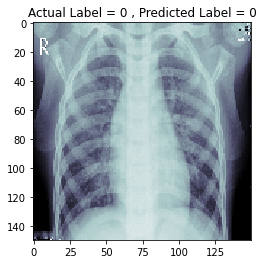
\includegraphics[width=200pt]{pictures/resultado_exemplo.png}
    \caption{Exemplo de resultado do modelo}
    \label{pic:resultado_modelo}
    \end{center}
\end{figure}


Os dados obtidos vêm, por padrão, com um gabarito anexado, o que possibilitou a comparação direta. Contudo, na aplicação prática, o resultado se limitaria à classe prevista pelo modelo.